\numberwithin{equation}{section}

\subsection{Histograms}
%\begin{frame}
  %\frametitle{Outline}
  %\tableofcontents[ currentsection ]
%\end{frame}

\begin{frame}{Description of Simulations}
We wrote code in C and MatLab that approximated our two-dimensional system of equations. 
	\begin{itemize}
		\item Ran both languages for $N = 10,000$ as a check
		\item Ran C for $N =45,000$ because MatLab is SLOW!
	\end{itemize}
\end{frame}


\begin{frame}{Results}
 

  \begin{columns}[t]
    \column{.5\textwidth} 
    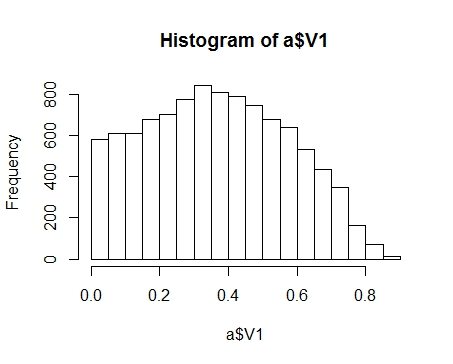
\includegraphics[width=6cm]{img/shrimpHistMATLAB} \\
		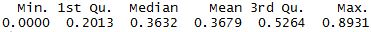
\includegraphics[width=5.5cm]{img/histSummML}
    \begin{center} Histogram from Matlab simulations \end{center}
    \column{.5\textwidth}
    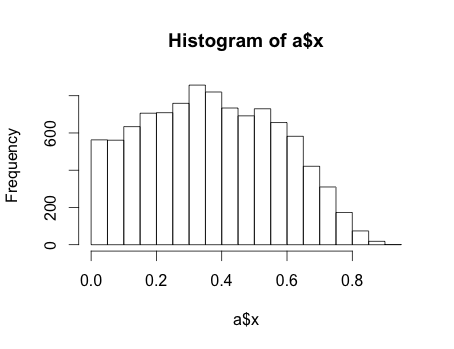
\includegraphics[width=6cm]{img/Rplot} \\
		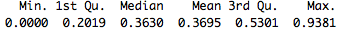
\includegraphics[width=5.5cm]{img/sumAMAN}
    \begin{center} Histogram from C simulations \end{center}
  \end{columns}


\end{frame}